\documentclass[11pt,a4paper]{article}

\usepackage[utf8]{inputenc}
\usepackage[T1]{fontenc}
\usepackage{lmodern}
\usepackage{microtype}
\usepackage[margin=2.5cm]{geometry}
\usepackage{amsmath,amssymb}
\usepackage{tikz}
\usetikzlibrary{ positioning, arrows.meta, calc, fit, shapes.geometric }
\usepackage{pgfplots}
\pgfplotsset{compat=1.16}
\usepackage{hyperref}
\usepackage{booktabs}
\usepackage{listings}
\usepackage{xcolor}

\definecolor{codegreen}{rgb}{0,0.6,0}
\definecolor{codegray}{rgb}{0.5,0.5,0.5}
\definecolor{codepurple}{rgb}{0.58,0,0.82}
\definecolor{backcolour}{rgb}{0.95,0.95,0.92}
\definecolor{accent}{HTML}{27ae60}
\definecolor{accent2}{HTML}{2980b9}
\definecolor{accent3}{HTML}{e67e22}

% headings and links carry the accent palette so the document reads as one piece
\usepackage{titlesec}
\titleformat{\section}{\Large\bfseries\color{accent2}}{\thesection}{0.6em}{}
\titleformat{\subsection}{\large\bfseries\color{accent2!80!black}}{\thesubsection}{0.6em}{}
\titlespacing*{\section}{0pt}{2.4ex plus 1ex minus .2ex}{1.1ex plus .2ex}
\hypersetup{colorlinks=true, linkcolor=accent2, urlcolor=accent2, citecolor=accent2,
            pdftitle={Quick IPT: Mathematics and Implementation of Hidden-Point Measurement},
            pdfauthor={EVKA Position Project}}

\lstset{
  backgroundcolor=\color{backcolour},
  commentstyle=\color{codegreen},
  keywordstyle=\color{magenta},
  numberstyle=\tiny\color{codegray},
  stringstyle=\color{codepurple},
  basicstyle=\ttfamily\footnotesize,
  breaklines=true,
  captionpos=b,
  keepspaces=true,
  numbers=left,
  numbersep=5pt,
  showspaces=false,
  showstringspaces=false,
  tabsize=2
}

\newcommand{\M}{\mathbf{M}}
\newcommand{\bP}{\mathbf{P}}
\newcommand{\bC}{\mathbf{C}}
\newcommand{\bu}{\mathbf{u}}
\newcommand{\bd}{\mathbf{d}}
\newcommand{\bx}{\mathbf{x}}
\newcommand{\beps}{\boldsymbol{\varepsilon}}
\newcommand{\R}{\mathbb{R}}
\newcommand{\norm}[1]{\left\lVert #1 \right\rVert}

\title{Quick IPT --- Mathematics and Implementation\\of Hidden-Point Measurement\\[4pt]
\large A detailed companion to the EVKA Position IPT report}
\author{EVKA Position Project}
\date{\today}

\begin{document}
\maketitle

% ══════════════════════════════════════════════════════════════════════════════
\section{Introduction and problem statement}

The EVKA Position system measures a Cartesian point $(X,Y,Z)$ in millimetres from
three encoders: one draw-wire encoder for radius $r$ and two rotary encoders for
azimuth $\theta$ and elevation $\phi$. It reports a \textbf{3-DOF point}, not a
6-DOF pose --- there is no orientation sensor. Consequently a point behind an
obstacle, around a corner, or inside a recess cannot be reached by the tip
directly: the tip has no line of travel to it.

Quick IPT removes this restriction with a purely geometric trick. Attach a rigid
pen to the draw-wire body so that the wire couples to the pen at a fixed offset $L$
from the pen \emph{tip}. Hold the tip motionless on the hidden target $\bP$ and
sweep the handle through a wide cone. Because the tip does not move, the wire-side
attachment point $\M_i$ that the sensor actually measures is always exactly $L$
away from $\bP$:
\begin{equation}
  \norm{\M_i - \bP} = L \qquad \text{for every sample } i .
  \label{eq:core}
\end{equation}
Every $\M_i$ therefore lies on a sphere of radius $L$ centred on the target.
Fitting that sphere to the measured point cloud recovers its centre $\bP$ --- the
hidden target --- and, if $L$ is treated as unknown, the radius simultaneously
\emph{self-calibrates} the pen offset.

\begin{center}
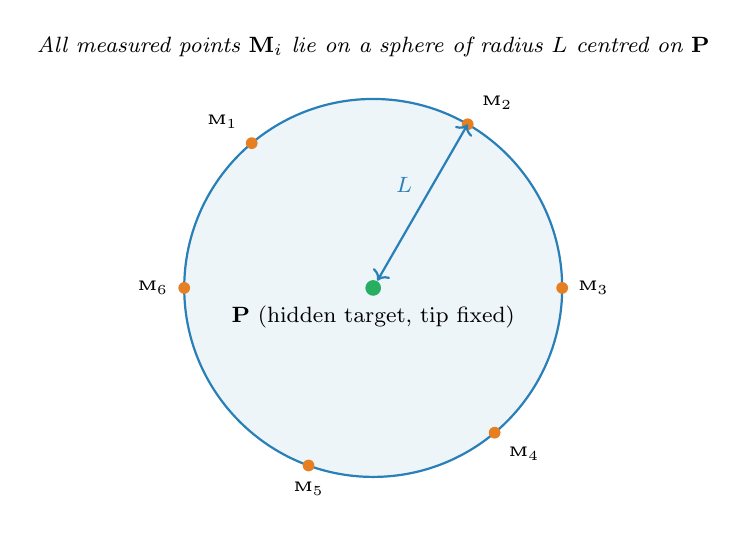
\begin{tikzpicture}[
  scale=1.0,
  every node/.style={font=\small},
  sphere/.style={circle, draw=accent2, fill=accent2!8, thick,
                 minimum width=4.8cm, minimum height=4.8cm},
  target/.style={circle, fill=accent, inner sep=2pt},
  mpt/.style={circle, fill=accent3, inner sep=1.5pt},
]
  \node[sphere] (s) at (0,0) {};
  \node[target, label={[font=\footnotesize]below:$\bP$ (hidden target, tip fixed)}] (P) at (0,0) {};
  \node[mpt, label={[font=\tiny]above left:$\M_1$}] at (130:2.4) {};
  \node[mpt, label={[font=\tiny]above right:$\M_2$}] at (60:2.4) {};
  \node[mpt, label={[font=\tiny]right:$\M_3$}] at (0:2.4) {};
  \node[mpt, label={[font=\tiny]below right:$\M_4$}] at (-50:2.4) {};
  \node[mpt, label={[font=\tiny]below:$\M_5$}] at (-110:2.4) {};
  \node[mpt, label={[font=\tiny]left:$\M_6$}] at (180:2.4) {};
  \draw[<->, thick, accent2] (P) -- (60:2.4)
    node[midway, above left, font=\footnotesize] {$L$};
  \node[above=0.4cm of s, font=\footnotesize\itshape]
    {All measured points $\M_i$ lie on a sphere of radius $L$ centred on $\bP$};
\end{tikzpicture}
\end{center}

The single sample is useless on its own --- $\bP$ could be anywhere on a sphere
around it --- which is exactly why the method needs \emph{many} samples spread over
a wide cone. Sections~\ref{sec:model}--\ref{sec:cond} make that intuition precise:
the recoverability of $\bP$ is governed by the angular spread of the samples, and
a small cone is a nearly flat patch of a large sphere that pins the centre only
weakly.

% ══════════════════════════════════════════════════════════════════════════════
\section{Research context and related work}
\label{sec:context}

\paragraph{Prodim Proliner and the patent.}
The method was pioneered by \textbf{Prodim International} for the Proliner family of
draw-wire 3D templating scanners and is protected by \textbf{US~9{,}267{,}794~B2}
(Teune \& Janssen, ``Method of determining a target spatial coordinate using an
apparatus comprising a movable hand-held probe and a portable base unit'').  The
patent describes precisely the two solver modes used here. With a \emph{known}
offset it forms, for each orientation, a virtual sphere ``having centres
corresponding to the spatial coordinates of the attachment point, wherein radii of
the spheres equal a crow flying distance between the attachment point and a pointing
tip,'' and takes the target at their intersection --- this is the fixed-radius
trilateration of \S\ref{sec:trilat}. With an \emph{unknown} offset it instead
determines ``one virtual sphere spanned by the coordinates of each attachment
point,'' whose centre ``being the target spatial coordinate'' --- the
self-calibrating sphere fit of \S\ref{sec:coope}--\ref{sec:gn}. EVKA Position has
the same sensor topology (one wire $+$ two angle encoders), so the method transfers
directly and needs \textbf{no firmware change}.

\paragraph{Pivot calibration.}
Mathematically, IPT is identical to \emph{pivot calibration}, a standard problem in
surgical navigation and robotics: find the fixed tip of a tracked tool by pivoting
it about a stationary point. Yaniv's survey ``Which Pivot Calibration?''
(SPIE 2015) compares three formulations --- geometry-based \emph{sphere fitting}
(SF), an \emph{algebraic one-step} (AOS), and an \emph{algebraic two-step} (ATS)
estimator --- and finds that algebraic formulations seeded by, or combined with, a
geometric refinement are more precise and accurate than a naive sphere fit
(reporting $\sim\!0.25$--$0.35$\,mm on optical trackers). Our solver follows exactly
that recommended two-stage pattern: an algebraic seed (\S\ref{sec:coope} or
\S\ref{sec:trilat}) followed by a Gauss--Newton geometric refinement
(\S\ref{sec:gn}). The same problem appears in robotics as \emph{tool-centre-point
(TCP) calibration}.

\paragraph{Algebraic sphere fitting.}
The linear-least-squares sphere fit we seed with is the sphere analogue of Coope's
circle fit (``Circle fitting by linear and nonlinear least squares,'' JOTA 1993):
linearise the sphere equation by absorbing the quadratic centre term into a single
extra unknown, solve one linear system, then optionally refine.

\paragraph{Dilution of precision.}
The dependence of the target error on the \emph{shape} of the sweep, not just the
noise level, is dilution of precision --- the same phenomenon that makes a GNSS fix
poor when the visible satellites are clustered in one part of the sky. We make this
quantitative in \S\ref{sec:cond} through the condition number of a geometric
Jacobian of outward unit vectors, directly analogous to the geometry matrix behind
GDOP.

% ══════════════════════════════════════════════════════════════════════════════
\section{Geometric model and formulation}
\label{sec:model}

Write the measured attachment points as
\begin{equation}
  \M_i \;=\; \bP + L\,\bd_i + \beps_i, \qquad i = 1,\dots,n,
  \label{eq:meas}
\end{equation}
where $\bP \in \R^3$ is the hidden target, $L>0$ the (possibly unknown) pen offset,
$\bd_i \in \R^3$ a unit vector from tip to attachment set by the operator's hand
orientation on sample $i$, and $\beps_i$ the sensor error. We model $\beps_i$ as
zero-mean, approximately isotropic with standard deviation $\sigma$ per axis; on
real hardware $\sigma$ bundles encoder quantisation, the exponential-moving-average
output filter, and mechanical play.

Dropping the noise, \eqref{eq:meas} gives the exact constraint \eqref{eq:core}. The
unknowns are $\bP$ (three components) and $L$ (one), so \textbf{four} in the
self-calibrating case and \textbf{three} when $L$ is supplied. Each sample
contributes one scalar equation, so four points define a sphere in principle. In
practice the solver requires
\[
  n \;\ge\; \texttt{MIN\_POINTS} = 8,
\]
because a real, noisy, partial arc needs redundancy for a stable fit --- four points
on a small cap are catastrophically ill-conditioned (\S\ref{sec:cond}).

All coordinates are in the \textbf{sensor origin frame}: the boot zero-point set by
\texttt{setZeroPoint()}, in millimetres, the same frame as the live $X/Y/Z$ readout.
The recovered $\bP$ inherits that frame; it is not a world coordinate.

% ══════════════════════════════════════════════════════════════════════════════
\section{The three estimators}
\label{sec:estimators}

The solver combines three classical estimators. Two are linear and closed-form and
serve as seeds; the third is an iterative geometric refinement that produces the
final answer and the residual used for quality gating. Each subsection ends with the
function in \texttt{tools/ipt/solver.py} that implements it.

% ────────────────────────────────────────────────────────────────
\subsection{[A] Coope algebraic linear least squares}
\label{sec:coope}

Start from the squared constraint and expand:
\begin{equation}
  \norm{\M - \bC}^2 = r^2
  \;\Longleftrightarrow\;
  \norm{\M}^2 - 2\,\M^\top\bC + \norm{\bC}^2 = r^2 .
\end{equation}
The term $\norm{\bC}^2$ is what makes this nonlinear in $\bC$. Coope's device is to
absorb it into a single scalar unknown $g \equiv r^2 - \norm{\bC}^2$, leaving an
equation that is \emph{linear} in the four unknowns $(\bC, g)$:
\begin{equation}
  2\,\M_i^\top \bC + g = \norm{\M_i}^2 .
  \label{eq:coope-lin}
\end{equation}
Stacking all $n$ samples,
\begin{equation}
  \underbrace{\begin{bmatrix} 2\M_1^\top & 1 \\ \vdots & \vdots \\ 2\M_n^\top & 1\end{bmatrix}}_{A}
  \underbrace{\begin{bmatrix}\bC \\ g\end{bmatrix}}_{\bx}
  =
  \underbrace{\begin{bmatrix}\norm{\M_1}^2 \\ \vdots \\ \norm{\M_n}^2\end{bmatrix}}_{b},
  \qquad
  \bx = \arg\min_\bx \norm{A\bx - b}^2 ,
  \label{eq:coope-ls}
\end{equation}
solved by one linear least squares. The radius is recovered as
$r = \sqrt{g + \norm{\bC}^2}$.

\paragraph{Centering.}
In this workspace $\norm{\M_i} \sim 10^3$\,mm, so the coordinate columns of $A$ are
$\sim\!10^3$ while the constant column is $1$: a scale mismatch of a thousand that
inflates $\operatorname{cond}(A)$ for a reason that has nothing to do with the
measurement geometry. The fix is to subtract the cloud mean $\bar\M$ before
solving, so the (centred) coordinate columns and the constant column are
comparable, then add $\bar\M$ back to the recovered centre. This is exactly what the
code does:

\begin{lstlisting}[language=Python]
mean = M.mean(axis=0)
Mc = M - mean
A = np.hstack([2 * Mc, np.ones((len(Mc), 1))])
b = np.sum(Mc ** 2, axis=1)
sol, _, _, sv = lstsq(A, b, rcond=None)
Cc = sol[:3]
C = Cc + mean                            # add the mean back
r = np.sqrt(max(0.0, sol[3] + Cc @ Cc))  # guard neg. radicand
\end{lstlisting}

\noindent $\Rightarrow$ \texttt{fit\_sphere\_algebraic(M)} $\to (\bC, r,
\operatorname{cond})$. This is the seed for the self-calibrating path, and its
radius $r$ is reported separately as \texttt{L\_fit}, an \emph{independent} estimate
of the pen length that can be compared against a user-supplied $L$ as a sanity check.

% ────────────────────────────────────────────────────────────────
\subsection{[B] Fixed-radius differencing (trilateration)}
\label{sec:trilat}

When the pen length $L$ is known, the radius is no longer an unknown and a better
conditioned linear solve is available. Expand the constraint for two samples $i$
and $0$ and subtract:
\begin{align}
  \norm{\M_i}^2 - 2\,\M_i^\top\bP + \norm{\bP}^2 &= L^2, \\
  \norm{\M_0}^2 - 2\,\M_0^\top\bP + \norm{\bP}^2 &= L^2.
\end{align}
Both the quadratic term $\norm{\bP}^2$ \emph{and} the (equal) radius $L^2$ cancel,
leaving a relation linear in $\bP$ alone:
\begin{equation}
  2\,(\M_i - \M_0)^\top \bP \;=\; \norm{\M_i}^2 - \norm{\M_0}^2 ,
  \qquad i = 1,\dots,n-1 .
  \label{eq:trilat}
\end{equation}
This is trilateration: each equation says $\bP$ is equidistant (namely $L$) from
$\M_i$ and $\M_0$, i.e.\ it lies on the radical plane between the two spheres.
Because the radius unknown has been eliminated, the $3\times3$ system is far better
conditioned than \eqref{eq:coope-ls}; the value of $L$ never even enters, only the
fact that it is the \emph{same} for every point.

\begin{lstlisting}[language=Python]
M0 = M[0]
A = 2 * (M[1:] - M0)
d = np.sum(M[1:] ** 2, axis=1) - np.sum(M0 ** 2)
p, _, _, sv = lstsq(A, d, rcond=None)
\end{lstlisting}

\noindent $\Rightarrow$ \texttt{trilaterate\_fixed\_radius(M)} $\to (\bP,
\operatorname{cond})$, needing $n \ge 4$. It is the seed for the known-$L$ path.

% ────────────────────────────────────────────────────────────────
\subsection{[C] Gauss--Newton geometric refinement}
\label{sec:gn}

The linear estimators [A] and [B] minimise an \emph{algebraic} residual --- the
error in \eqref{eq:coope-lin}/\eqref{eq:trilat} --- which weights each point by a
factor that grows with its distance from the centre and is therefore biased on
noisy, partial arcs. The statistically correct objective, and the one that yields
the residual we report, is the \emph{geometric} residual: the signed Euclidean
distance from each point to the fitted sphere surface,
\begin{equation}
  f_i(\bC, r) \;=\; \norm{\M_i - \bC} - r .
  \label{eq:geores}
\end{equation}
Under isotropic Gaussian noise $\beps_i$, minimising $\sum_i f_i^2$ is the maximum-
likelihood estimate of $(\bC, r)$. We minimise it with Gauss--Newton. Let
\begin{equation}
  \bu_i \;=\; \frac{\M_i - \bC}{\norm{\M_i - \bC}}
\end{equation}
be the outward unit vector at sample $i$. The partial derivatives of
\eqref{eq:geores} are
\begin{equation}
  \frac{\partial f_i}{\partial \bC} = -\bu_i^\top, \qquad
  \frac{\partial f_i}{\partial r} = -1 ,
\end{equation}
so the Jacobian row is $\big[-\bu_i^\top,\ -1\big]$. Each iteration solves the
linearised least-squares step $J\,\Delta = -\mathbf{f}$ and updates
$[\bC; r] \mathrel{+}= \Delta$:
\begin{equation}
  J = \begin{bmatrix} -\bu_1^\top & -1 \\ \vdots & \vdots \\ -\bu_n^\top & -1 \end{bmatrix}
  \in \R^{n\times 4},
  \qquad
  \Delta = \arg\min_\Delta \norm{J\Delta + \mathbf{f}}^2 .
\end{equation}
When $L$ is known the radius is held fixed: the last column of $J$ is dropped, the
step solves for $\Delta\bC$ only, and $J \in \R^{n\times 3}$. The implementation
floors $\norm{\M_i-\bC}$ at $10^{-9}$ (a point exactly at the centre has no defined
direction), breaks if a step exceeds $10^4$ (divergence guard), and stops when
$\norm{\Delta} < 10^{-9}$:

\begin{lstlisting}[language=Python]
diff = M - C
dist = np.maximum(norm(diff, axis=1), 1e-9)  # guard /0
u = diff / dist[:, None]
f = dist - r
J = np.hstack([-u, -np.ones((len(M), 1))])   # -u only, if fixed_r
dx, _, _, _ = lstsq(J, -f, rcond=None)
C = C + dx[:3];  r = r + dx[3]               # update
\end{lstlisting}

\noindent $\Rightarrow$ \texttt{refine\_nonlinear(M, C0, r0=..., fixed\_r=...)} $\to
(\bC, r, \text{rms})$, where the returned root-mean-square of $\{f_i\}$ is the
quality metric of \S\ref{sec:gates}.

% ────────────────────────────────────────────────────────────────
\subsection{The pipeline: \texttt{solve\_ipt}}
\label{sec:pipeline}

\texttt{solve\_ipt(M, L=None)} wires the three estimators into the two-stage,
seed-then-refine pattern recommended by Yaniv:

\begin{center}
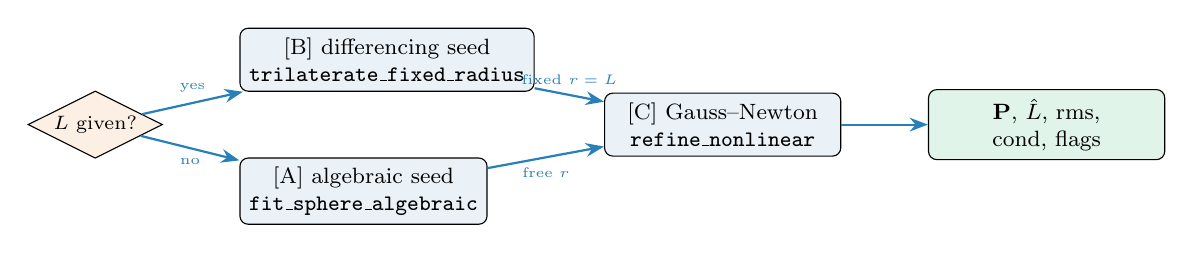
\begin{tikzpicture}[
  node distance=0.7cm and 1.1cm,
  mod/.style={draw, rounded corners=3pt, fill=accent2!10,
              minimum width=3.0cm, minimum height=0.8cm, align=center, font=\footnotesize},
  dec/.style={draw, diamond, aspect=2, fill=accent3!12, align=center, font=\scriptsize, inner sep=1pt},
  ar/.style={-Stealth, thick, accent2},
]
  \node[dec] (q) {$L$ given?};
  \node[mod, above right=0.2cm and 1.4cm of q] (tri) {[B] differencing seed\\\texttt{trilaterate\_fixed\_radius}};
  \node[mod, below right=0.2cm and 1.4cm of q] (alg) {[A] algebraic seed\\\texttt{fit\_sphere\_algebraic}};
  \node[mod, right=5.6cm of q] (gn) {[C] Gauss--Newton\\\texttt{refine\_nonlinear}};
  \node[mod, right=of gn, fill=accent!14] (out) {$\bP$, $\hat L$, rms,\\cond, flags};
  \draw[ar] (q) -- node[above,font=\tiny]{yes} (tri);
  \draw[ar] (q) -- node[below,font=\tiny]{no} (alg);
  \draw[ar] (tri) -- node[above,font=\tiny]{fixed $r=L$} (gn);
  \draw[ar] (alg) -- node[below,font=\tiny]{free $r$} (gn);
  \draw[ar] (gn) -- (out);
\end{tikzpicture}
\end{center}

\begin{itemize}
\item \textbf{Self-calibrating} ($L=\texttt{None}$): algebraic seed [A] $\to$
  Gauss--Newton [C] with free radius. $\hat L$ is the fitted pen length; it should
  match the physical pen within a few mm.
\item \textbf{Known $L$}: differencing seed [B] $\to$ Gauss--Newton [C] with the
  radius held at $L$. $\hat L = L$ (the value used); \texttt{L\_fit} is the
  independent algebraic radius from [A], reported so the operator can check the
  entered length against the data.
\end{itemize}

Because $n \ge \texttt{MIN\_POINTS} = 8$ is enforced first, the $n \ge 4$
precondition of [B] always holds. The return dictionary carries
\[
  \{\,\texttt{ok},\ \bP,\ \texttt{L\_hat},\ \texttt{L\_fit},\ \texttt{rms\_resid},\
     \texttt{cond},\ \texttt{n\_points},\ \texttt{slip\_warning},\ \texttt{geom\_warning}\,\}.
\]

% ══════════════════════════════════════════════════════════════════════════════
\section{Conditioning and dilution of precision}
\label{sec:cond}

The residual RMS tells you whether the points lie on \emph{a} sphere; it does
\textbf{not} tell you whether that sphere's centre is well determined. A small cap
of a large sphere fits its points beautifully (tiny RMS) yet leaves the centre
almost free to slide along the sweep axis. The quantity that captures this is the
conditioning of the geometric Jacobian.

\paragraph{Why the algebraic condition number is the wrong indicator.}
Centering the cloud before the algebraic fit (\S\ref{sec:coope}) deliberately
removes the scale-driven part of $\operatorname{cond}(A)$ --- which was the whole
point of centering --- so the algebraic condition number no longer reflects sweep
geometry. Using it as a ``sweep wider'' cue would be meaningless.

\paragraph{The geometric Jacobian.}
Instead, use the Jacobian of outward unit vectors evaluated at the solution,
\begin{equation}
  J \;=\;
  \begin{bmatrix} \bu_1^\top & 1 \\ \vdots & \vdots \\ \bu_n^\top & 1 \end{bmatrix}
  \in \R^{n\times 4}
  \quad\text{(unit vectors, plus a ones column)},
  \qquad
  \kappa \;=\; \operatorname{cond}(J) = \frac{\sigma_{\max}(J)}{\sigma_{\min}(J)} .
  \label{eq:geojac}
\end{equation}
Near the solution the linearised model is $\mathbf{f} \approx J\,\delta$ with
$\delta = [\delta\bC; \delta r]$, so the parameter perturbation induced by
measurement noise is $\delta \approx (J^\top J)^{-1} J^\top \beps$, giving the
first-order covariance
\begin{equation}
  \operatorname{Cov}(\hat\bP) \;\approx\; \sigma^2\,\big[(J^\top J)^{-1}\big]_{1:3,\,1:3} .
  \label{eq:cov}
\end{equation}
When the unit vectors $\bu_i$ cluster (a narrow cone) they become nearly parallel
to one another and to the constant column, $J^\top J$ approaches singularity, and
$(J^\top J)^{-1}$ blows up along the sweep axis. $\kappa$ is a scalar summary of
that blow-up: a \textbf{dilution-of-precision} number, mathematically the same
geometry factor as the GDOP of a GNSS fix (unit vectors to satellites) or the
condition of a pivot-calibration design matrix.

The same 4-column form \eqref{eq:geojac} is used for both the self-calibrating and
known-$L$ paths so the thresholds stay consistent; it is monotone with angular
spread either way.

\begin{lstlisting}[language=Python]
u = diff / np.maximum(norm(diff, axis=1), 1e-9)[:, None]
J = np.hstack([u, np.ones((len(M), 1))])
return float(np.linalg.cond(J))                  # geometry_cond(M, C)
\end{lstlisting}

\paragraph{Averaging.}
For a fixed geometry, \eqref{eq:cov} scales as $\sigma^2/n$ through the $J^\top J$
accumulation, so the target error falls roughly as $\sigma/\sqrt{n}$. More points
average down noise; they do \emph{not} fix bad geometry --- only a wider sweep
does. Section~\ref{sec:study} confirms both trends numerically.

% ══════════════════════════════════════════════════════════════════════════════
\section{Quality gates}
\label{sec:gates}

Two independent, heuristic gates translate the fit into an operator verdict. They
are deliberately generous: the wire encoder plus EMA filter is coarser than the
sub-mm optical trackers of the pivot-calibration literature (Yaniv reports
$0.3$--$0.8$\,mm there), so mm-scale bands are appropriate and should be re-tuned on
real hardware.

\begin{center}
\begin{tabular}{@{}lll@{}}
\toprule
Flag & Metric & Bands \\
\midrule
\textbf{slip\_warning} & RMS geometric residual &
  \texttt{ok} $<2$\,mm,\;\; \texttt{warn} $2$--$5$\,mm,\;\; \texttt{reject} $>5$\,mm \\[3pt]
\textbf{geom\_warning} & Geometric Jacobian $\kappa$ &
  \texttt{ok} $<150$,\;\; \texttt{warn} $150$--$1500$,\;\; \texttt{block} $>1500$ \\
\bottomrule
\end{tabular}
\end{center}

\begin{itemize}
\item \textbf{RMS residual} (\texttt{RESIDUAL\_ACCEPT\_MM}\,$=2$,
  \texttt{RESIDUAL\_REJECT\_MM}\,$=5$) rises when the tip slips off the target during
  the sweep, because the points then no longer lie on a single sphere. It flags
  slip but cannot correct it --- re-measure.
\item \textbf{Geometry $\kappa$} (\texttt{COND\_WARN}\,$=150$,
  \texttt{COND\_BLOCK}\,$=1500$) rises when the sweep is too small. As
  \S\ref{sec:study} shows, $\kappa=150$ corresponds to $\sim\!18^\circ$ of half-angle
  ($\sim\!1.6$\,mm error) and $\kappa=1500$ to $\sim\!5^\circ$ ($\sim\!20$\,mm error).
\end{itemize}

The GUI combines them into one verdict: \texttt{reject} if either
$\texttt{slip}=\texttt{reject}$ or $\texttt{geom}=\texttt{block}$; else
\texttt{warn} if either warns; else \texttt{ok}.

% ══════════════════════════════════════════════════════════════════════════════
\section{Implementation}
\label{sec:impl}

The entire feature is a host-side Python package, \texttt{tools/ipt/}; the ESP32
firmware is untouched. The tool subscribes to the existing 20\,Hz position stream,
buffers a swept point cloud, and runs \texttt{solve\_ipt} on demand.

\begin{center}
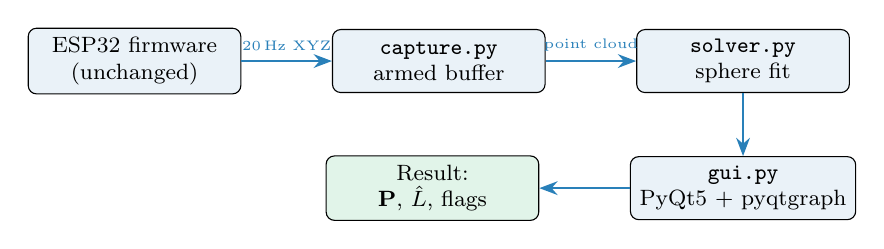
\begin{tikzpicture}[
  node distance=0.8cm and 1.15cm,
  mod/.style={draw, rounded corners=3pt, fill=accent2!10,
              minimum width=2.7cm, minimum height=0.8cm, align=center, font=\footnotesize},
  ar/.style={-Stealth, thick, accent2},
]
  \node[mod] (firm) {ESP32 firmware\\(unchanged)};
  \node[mod, right=of firm] (cap) {\texttt{capture.py}\\armed buffer};
  \node[mod, right=of cap] (sol) {\texttt{solver.py}\\sphere fit};
  \node[mod, below=of sol] (gui) {\texttt{gui.py}\\PyQt5 + pyqtgraph};
  \node[mod, left=of gui, fill=accent!14] (out) {Result:\\$\bP$, $\hat L$, flags};
  \draw[ar] (firm) -- node[above, font=\tiny] {20\,Hz XYZ} (cap);
  \draw[ar] (cap) -- node[above, font=\tiny] {point cloud} (sol);
  \draw[ar] (sol) -- (gui);
  \draw[ar] (gui) -- (out);
\end{tikzpicture}
\end{center}

\subsection{Transport asymmetry and the pairing state machine}

The firmware emits different line formats on the two transports:
\begin{itemize}
\item \textbf{Serial} --- one self-contained line per cycle, carrying position and
  validity together:
  \begin{center}\ttfamily\footnotesize
  DATA,$x$,$y$,$z$,$r$,$\theta$,$\phi$,is\_valid,frame\_count,ts\_ms
  \end{center}
  parsed by \texttt{parse\_line} into a \texttt{ParsedFrame}; non-finite fields make
  the parse return \texttt{None}, and \texttt{DataStore.push} drops any frame with
  \texttt{is\_valid==0} before it reaches the buffer.
\item \textbf{TCP} --- position and validity arrive as \emph{two separate lines}:
  \begin{center}\ttfamily\footnotesize
  X$x$,Y$y$,Z$z$ \qquad then \qquad SENSOR,$r$,$\theta$,$\phi$,is\_valid,frame\_count
  \end{center}
  The \texttt{X..,Y..,Z..} line has the coordinates but no validity; the following
  \texttt{SENSOR,..} line has validity but no coordinates.
\end{itemize}

The capture buffer therefore runs a tiny two-state pairing machine on the TCP path:
an XYZ line is \emph{stashed} (committing nothing), and the next SENSOR line
consumes the stash, committing the point through the acceptance gate only if
\texttt{is\_valid} is set. Any intervening non-XYZ/non-SENSOR line leaves the stash
untouched; \texttt{disarm()}/\texttt{clear()} reset it so a half-received pair never
straddles a re-arm.

\begin{lstlisting}[language=Python]
xyz = parse_xyz_line(line)
if xyz is not None:
    self._pending_xyz = (xyz.x_mm, xyz.y_mm, xyz.z_mm)   # stash; commit later
    return False
sensor = parse_sensor_line(line)
if sensor is not None:
    pending = self._pending_xyz
    self._pending_xyz = None                    # consume the slot
    if sensor.is_valid and pending is not None:
        return self._accept(*pending)           # commit paired point
return False
\end{lstlisting}

\subsection{Acceptance gates}

Every candidate point passes three gates in \texttt{IptCapture.\_accept} before it
enters the cloud:
\begin{enumerate}
\item \textbf{Armed} --- reject unless capture is armed.
\item \textbf{Finite} --- reject any non-finite coordinate (belt-and-braces on the
  TCP path, where floats are parsed straight off the wire).
\item \textbf{Dedup} --- reject if the squared displacement from the last accepted
  point is below \texttt{DEFAULT\_MIN\_DISP\_MM}$^2 = (1\,\text{mm})^2$. At 20\,Hz a
  momentarily still handle emits many near-identical frames; only points that moved
  $\ge 1$\,mm are kept. The threshold is stored squared to avoid a square root per
  sample.
\end{enumerate}

\subsection{GUI and threading}

\texttt{gui.py} (\texttt{IptWindow}) renders three 2D projections (top $XY$, front
$XZ$, side $YZ$) using \texttt{pyqtgraph} rather than a 3D GL view, for portability
on headless / Wayland / VM setups. Transports run on daemon threads that only
enqueue raw lines (TCP) or push parsed frames to a thread-safe \texttt{DataStore}
(serial); a 40\,ms (25\,Hz) \texttt{QTimer} on the GUI thread drains the queue,
feeds the capture buffer, and redraws. All buffer mutation and all plotting happen
on the GUI thread --- the capture methods are never called from a transport
callback. The operator flow is \textbf{CONNECT $\to$ ARM $\to$ sweep $\to$ STOP
$\to$ SOLVE}; SOLVE draws the fitted circle of radius $\hat L$ on each projection and
an orange marker at $\bP$, and prints the two quality flags.

\subsection{Solver $\leftrightarrow$ mathematics}

\begin{center}
\begin{tabular}{@{}lll@{}}
\toprule
Function (\texttt{solver.py}) & Section & Role \\
\midrule
\texttt{fit\_sphere\_algebraic}     & \S\ref{sec:coope} & [A] Coope linear seed; also gives \texttt{L\_fit} \\
\texttt{trilaterate\_fixed\_radius} & \S\ref{sec:trilat} & [B] known-$L$ differencing seed \\
\texttt{refine\_nonlinear}          & \S\ref{sec:gn}     & [C] Gauss--Newton; returns final $\bP$ and RMS \\
\texttt{geometry\_cond}             & \S\ref{sec:cond}   & DOP indicator $\kappa$ \\
\texttt{solve\_ipt}                 & \S\ref{sec:pipeline} & pipeline + gating \\
\texttt{sample\_directions}         & \S\ref{sec:study}  & synthetic golden-spiral sweep (demo/tests/study) \\
\bottomrule
\end{tabular}
\end{center}

\subsection{Self-check and tests}

Running \texttt{python -m tools.ipt.solver} synthesises 12 points on a $35^\circ$
golden spiral at $L=400$\,mm with $0.1$\,mm noise and prints, reproducibly,
$\hat\bP=[1200.101,\,-450.051,\,300.389]$, $\hat L=399.596$\,mm, rms $=0.073$\,mm,
$\kappa=35$, both flags \texttt{ok}, and a target error of $0.405$\,mm --- proving
the math before any hardware is attached. The offline pytest suite
(\texttt{tools/ipt/tests/}) asserts, among others: self-cal target error $<2$\,mm
and $\hat L$ within $1$\,mm; the known-$L$ path within $2$\,mm; that a
$5$\,mm tip wander raises \texttt{slip\_warning}; that a $2^\circ$ sweep raises
\texttt{geom\_warning}; that $n=7$ returns \texttt{ok:False} without crashing; the
$1$\,mm dedup boundary; and the TCP pairing with validity recovery.

% ══════════════════════════════════════════════════════════════════════════════
\section{Simulation study}
\label{sec:study}

To quantify the analysis of \S\ref{sec:cond}, \texttt{docs/reports/ipt/sim\_study.py}
runs the \emph{actual} \texttt{solve\_ipt} on synthetic clouds. Ground truth is
$\bP_\text{true}=[1200,-450,300]$\,mm and $L_\text{true}=400$\,mm; sweeps use the
same golden-spiral \texttt{sample\_directions} the operator's hand motion is modelled
on; each configuration is averaged over 16 independent noise realisations. The
reported error is $\norm{\hat\bP - \bP_\text{true}}$, self-calibrating (i.e.\ $L$
treated as unknown).

\subsection{Error and conditioning versus sweep half-angle}

\begin{table}[h]
\centering
\begin{tabular}{@{}rrrrr@{}}
\toprule
Half-angle & $\kappa$ (cond) & RMS (mm) & Target err (mm) & $\hat L$ err (mm) \\
\midrule
2$^\circ$  & 22684 & 0.076 & 181.751 & 181.689 \\
3$^\circ$  & 5549  & 0.076 & 59.490  & 59.433  \\
5$^\circ$  & 1850  & 0.076 & 20.490  & 20.436  \\
8$^\circ$  & 717   & 0.076 & 7.968   & 7.915   \\
12$^\circ$ & 317   & 0.076 & 3.554   & 3.500   \\
18$^\circ$ & 140   & 0.076 & 1.595   & 1.547   \\
25$^\circ$ & 71    & 0.076 & 0.836   & 0.789   \\
35$^\circ$ & 35    & 0.076 & 0.436   & 0.386   \\
50$^\circ$ & 16    & 0.077 & 0.225   & 0.169   \\
70$^\circ$ & 8     & 0.078 & 0.129   & 0.076   \\
\bottomrule
\end{tabular}
\caption{Target error, self-calibrated length error, sphere-fit RMS and geometric
condition number versus sweep half-angle ($n=12$, $\sigma=0.1$\,mm, 16 seeds).
Note the RMS is essentially flat --- the points always fit a sphere well --- while
the target error spans three orders of magnitude. RMS alone is blind to the
geometry; $\kappa$ tracks it.}
\label{tab:angle}
\end{table}

Table~\ref{tab:angle} is the central result. The residual RMS barely moves
($0.076$--$0.078$\,mm) across the whole range, yet the target error collapses from
$182$\,mm at a $2^\circ$ pinhole sweep to $0.13$\,mm at a generous $70^\circ$ cone.
This is dilution of precision made concrete: a good-looking fit (small RMS) can
still hide a badly located centre, and only $\kappa$ exposes it. The gate thresholds
land exactly where intended --- $\kappa=\texttt{COND\_BLOCK}=1500$ at $\sim\!5^\circ$
($\approx 20$\,mm error) and $\kappa=\texttt{COND\_WARN}=150$ at $\sim\!18^\circ$
($\approx 1.6$\,mm error).

\begin{figure}[h]
\centering
\begin{minipage}{0.48\textwidth}
\centering
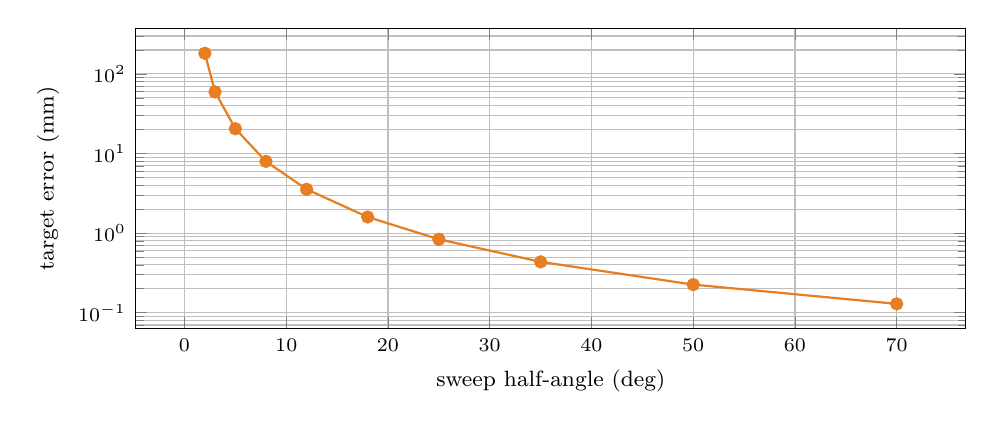
\begin{tikzpicture}
\begin{axis}[
  width=\textwidth, height=5.4cm, ymode=log,
  xlabel={sweep half-angle (deg)}, ylabel={target error (mm)},
  grid=both, tick label style={font=\scriptsize}, label style={font=\footnotesize},
]
\addplot[accent3, mark=*, thick] coordinates {(2,181.8) (3,59.49) (5,20.49) (8,7.968) (12,3.554) (18,1.595) (25,0.8364) (35,0.4358) (50,0.2255) (70,0.1292)};
\end{axis}
\end{tikzpicture}
\end{minipage}\hfill
\begin{minipage}{0.48\textwidth}
\centering
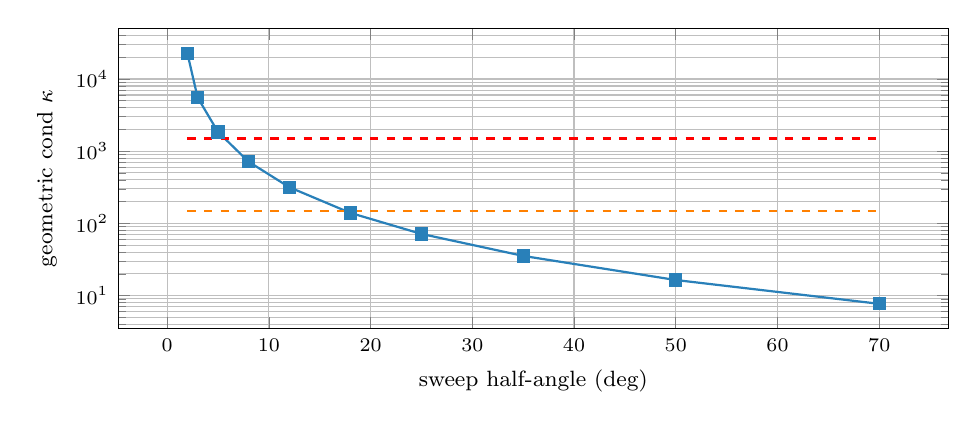
\begin{tikzpicture}
\begin{axis}[
  width=\textwidth, height=5.4cm, ymode=log,
  xlabel={sweep half-angle (deg)}, ylabel={geometric cond $\kappa$},
  grid=both, tick label style={font=\scriptsize}, label style={font=\footnotesize},
]
\addplot[accent2, mark=square*, thick] coordinates {(2,2.268e4) (3,5549) (5,1850) (8,716.9) (12,317.4) (18,139.8) (25,71.44) (35,35.43) (50,16.42) (70,7.685)};
\addplot[dashed, red, thick] coordinates {(2,1500) (70,1500)};
\addplot[dashed, orange, thick] coordinates {(2,150) (70,150)};
\end{axis}
\end{tikzpicture}
\end{minipage}
\caption{Left: target error (log scale) versus half-angle --- a small sweep is
catastrophic. Right: geometric condition number $\kappa$ (log scale) with the
\texttt{COND\_BLOCK}$=1500$ (red) and \texttt{COND\_WARN}$=150$ (orange) gate lines.}
\label{fig:angle}
\end{figure}

\subsection{Error versus noise and point count}

\begin{figure}[h]
\centering
\begin{minipage}{0.48\textwidth}
\centering
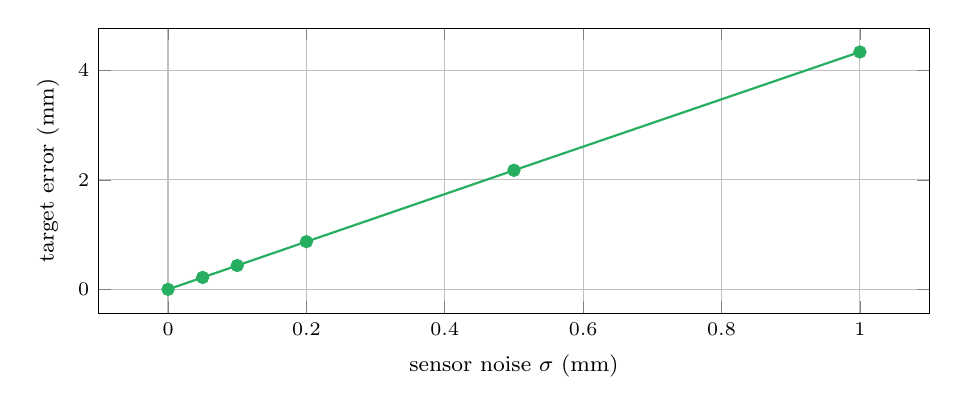
\begin{tikzpicture}
\begin{axis}[
  width=\textwidth, height=5.2cm,
  xlabel={sensor noise $\sigma$ (mm)}, ylabel={target error (mm)},
  grid=both, tick label style={font=\scriptsize}, label style={font=\footnotesize},
]
\addplot[accent, mark=*, thick] coordinates {(0,0) (0.05,0.218) (0.1,0.4358) (0.2,0.871) (0.5,2.174) (1,4.335)};
\end{axis}
\end{tikzpicture}
\end{minipage}\hfill
\begin{minipage}{0.48\textwidth}
\centering
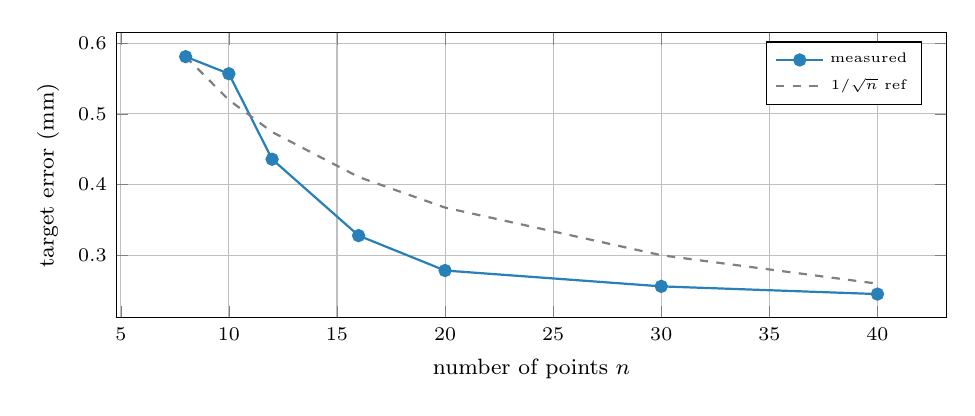
\begin{tikzpicture}
\begin{axis}[
  width=\textwidth, height=5.2cm,
  xlabel={number of points $n$}, ylabel={target error (mm)},
  grid=both, tick label style={font=\scriptsize}, label style={font=\footnotesize},
  legend style={font=\tiny, at={(0.97,0.97)}, anchor=north east},
]
\addplot[accent2, mark=*, thick] coordinates {(8,0.5809) (10,0.5567) (12,0.4358) (16,0.3278) (20,0.2784) (30,0.256) (40,0.2451)};
\addlegendentry{measured}
\addplot[dashed, gray, thick] coordinates {(8,0.5809) (10,0.5196) (12,0.4743) (16,0.4107) (20,0.3674) (30,0.3000) (40,0.2598)};
\addlegendentry{$1/\sqrt{n}$ ref}
\end{axis}
\end{tikzpicture}
\end{minipage}
\caption{Left: target error is \emph{linear} in the sensor noise $\sigma$
(half-angle $35^\circ$, $n=12$) --- doubling the noise doubles the error, as
\eqref{eq:cov} predicts. Right: target error versus point count (half-angle
$35^\circ$, $\sigma=0.1$\,mm) against a $1/\sqrt{n}$ reference; more samples average
the noise down but with diminishing returns.}
\label{fig:noise-n}
\end{figure}

Figure~\ref{fig:noise-n} confirms the two predictions of \S\ref{sec:cond}: for
fixed geometry the error is proportional to $\sigma$ (left), and it decreases
roughly as $1/\sqrt{n}$ with the number of points (right). The practical lesson is
the same as the analysis: \textbf{a wider sweep is worth far more than more
points}. Going from $12$ to $40$ points at $35^\circ$ cuts the error by about half;
going from $12^\circ$ to $35^\circ$ at $12$ points cuts it by a factor of eight.

The study script ends with a self-check \texttt{assert} (mean target error
$<2$\,mm and $\kappa<60$ at $35^\circ$, both flags \texttt{ok}) so a regression in the
solver or its numbers fails loudly. Regenerate all figures and tables with
\texttt{python docs/reports/ipt/sim\_study.py}.

% ══════════════════════════════════════════════════════════════════════════════
\section{Limitations}

\begin{itemize}
\item \textbf{3-DOF only.} EVKA Position returns a point, not a pose. IPT recovers
  the hidden \emph{point}, never the 6-DOF orientation of the pen.
\item \textbf{Tip slip.} The RMS residual flags it (\S\ref{sec:gates}) but cannot
  correct it. If the tip wanders off the target, the points stop lying on one
  sphere; re-measure.
\item \textbf{Sweep geometry.} Small or single-plane sweeps are ill-conditioned
  (Table~\ref{tab:angle}). The \texttt{geom\_warning} flag is the operator's cue to
  open the cone; in tight spaces a two-direction ``cross'' motion is the minimum
  viable substitute for a full spiral.
\item \textbf{Coordinate frame.} Results are in the sensor boot zero-point frame,
  not a world frame. Re-zeroing or moving the sensor invalidates a previously
  recovered target; transform externally if world coordinates are needed.
\item \textbf{Heuristic gates.} The $2/5$\,mm and $150/1500$ thresholds were tuned in
  simulation against a $0.1$\,mm noise model. Real hardware noise is larger and
  should be characterised, and the gates re-tuned, before field use.
\end{itemize}

% ══════════════════════════════════════════════════════════════════════════════
\section{Conclusion}

Quick IPT turns a 3-DOF draw-wire measuring system into a hidden-point probe with no
firmware change, by exploiting a single geometric fact: samples taken while the tip
is fixed lie on a sphere centred on the target. The estimator is a textbook
seed-then-refine pipeline --- an algebraic linear fit (Coope) or a fixed-radius
differencing solve for the seed, followed by a Gauss--Newton minimisation of the
geometric residual --- identical in structure to surgical and robotic pivot
calibration. The dominant error source is not sensor noise but sweep geometry:
the simulation study shows the target error spanning three orders of magnitude
across half-angle while the fit residual stays flat, which is exactly why the tool
gates on the condition number of a geometric Jacobian rather than on the residual
alone. Sweep wide.

% ══════════════════════════════════════════════════════════════════════════════
\section*{Intellectual property note}

The Quick IPT method is patented by Prodim International (US~9{,}267{,}794~B2,
EP~2{,}792{,}994~B1). This implementation is a technical reverse-engineering exercise
for research and educational purposes. The underlying mathematics --- sphere
fitting, trilateration, and pivot calibration --- is well established in the
literature. Commercial deployment may require licensing from Prodim.

\begin{thebibliography}{9}
\bibitem{teune2016}
  R.~Teune and A.~J.~Janssen,
  ``Method of determining a target spatial coordinate using an apparatus comprising
  a movable hand-held probe and a portable base unit, and a related apparatus,''
  US Patent 9{,}267{,}794~B2, 2016 (EP~2{,}792{,}994~B1).
\bibitem{yaniv2015}
  Z.~Yaniv,
  ``Which Pivot Calibration?,''
  \emph{Proc.\ SPIE Medical Imaging}, vol.~9415, 941527, 2015.
\bibitem{coope1993}
  I.~D.~Coope,
  ``Circle fitting by linear and nonlinear least squares,''
  \emph{J.\ Optim.\ Theory Appl.}, vol.~76, no.~2, pp.~381--388, 1993.
\bibitem{chen2017}
  E.~C.~S.~Chen \emph{et al.},
  ``Is pose-based pivot calibration superior to sphere fitting?,''
  \emph{Proc.\ SPIE Medical Imaging}, vol.~10135, 2017.
\bibitem{langley1999}
  R.~B.~Langley,
  ``Dilution of precision,''
  \emph{GPS World}, vol.~10, no.~5, pp.~52--59, 1999.
\end{thebibliography}

\end{document}
